\setcounter{section}{86}
\section{Алгоритм Штор—Вагнера поиска минимального глобального разреза.}

\textbf{Глобальный разрез} - разбиение множества V на два подмножества A и B, что $A, B \subset V; A, B \neq \varnothing; A \cap B = \varnothing; A \cup B = V$

\textbf{Величина (вес) разреза}: $c (S, T) = \sum_{u \in S, v\in T} c(u, v)$, где c(u, v) - capacity ребра из u в v (если нет такого ребра, то это ноль).

\textbf{Цель}: найти максимальный (или минимальный) глобальный разрез в G.

Поиск максимального глобального разреза в G - np-трудная. (Аналогично поиску максимальной клики/поиску Гамильтонова пути/цикла).

\textbf{Поиск минимального разреза во взвешенном неориентированном графе: наивный алгоритм.}

\begin{figure}[h]
\center{ 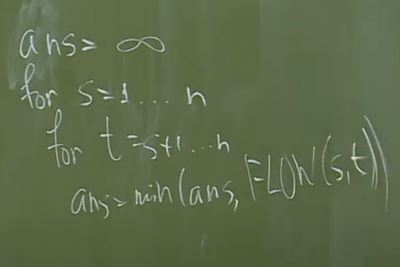
\includegraphics[height=4cm]{images/87-92_min_global}}
\end{figure}

(s - вершина, которая лежит в S, t - вершина, которая лежит в T). Для неориентированных графов можно считать, что вершина 1 всегда лежит в s, тогда s = 1, for t = 2, ..., n).

Асимптотика: n раз запустить поток, где $n = |V|$; поток за Диница считается за $V^2E$. Итого: $V^3E$.

\textbf{Замечание}. Если граф невзвешенный, то алгоритм Диница работает быстрее. \\

\textbf{Утверждение 1}. Пусть $a_1 = 1$, $A_i = \{a_1, \dots, a_i \}$. Тогда $a_{i+1}$ - вершина $\notin A_i$ с максимальным значением суммы рёбер до вершин из $A_i$: $c(\{v\}, A_i)$. $A_n = \{ 1, 2, \dots, n \}$. Тогда min разрез между $a_n$ и $a_{n-1}$ есть $(\{a_n\}, V\backslash \{a_n\})$. 

\textbf{Алгоритм Штор-Вагнера}.

Тогда min разрез из утверждения выше либо искомый ответ, либо $a_n, a_{n-1}$ можно положить в одну долю ("склеить": суммировать расстояния до оставшихся вершин), тогда рано или поздно найдём нужный разрез такими склеиваниями и проверками, \textbf{то есть, по сути, запускаем n-1 раз, склеивая вершины}.

\textbf{Асимптотика}: $O(V^3)$, потому что n раз запускаем эту процедуру поиска. (Что-то похожее на алгоритм Прима). Нахождение вершины с наибольшей w за O(n), n-1 фаза по n-1 итерации в каждой. В итоге имеем $O(n^3)$. Применяя фибоначчиевы или двоичные кучи, можно добиться асимптотик $O(nm+n^2logn)$ или $O(nmlogn+n^2)$ соответственно. \href{shorturl.at/hzM04}{Ссылочка}\\

\textbf{Докажем утверждение 1}: пусть это не так. Тогда рассмотрим С - настоящий минимальный разрез, $C = (S, T)$. Назовём $a_i$ - активной, если $a_{i-1}$ лежит в другой части вершин (вместо S - T, вместо T - S). Тогда для каждой активной $a_i$ $c(\{a_i\}, A_{i-1}) \leqslant c(S\cap A_i, T \cap A_i)$.

Пусть $a_j$ - первая активная вершина. Тогда все предыдущие лежат в одной половине, $a_j$ - в другой, т.е. $c(\{a_j\}, A_{j-1})$ - сумма рёбер из $a_j$ в другие рёбра; $c(S\cap A_j, T \cap A_j)$ - то же самое. База тривиальна, выполняется равенство: смотри картинку ниже. \\

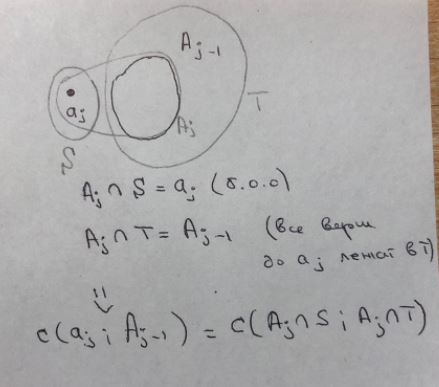
\includegraphics[height=4cm]{images/87-92_base}

По индукции: пусть верно для предыдущих активных вершин, $a_u, a_v$ - две последовательные активные вершины, т.е. вершины $[a_u, a_v)$ - в одной доле. Тогда $c(\{a_v\}, A_{v-1}) = c(\{a_v\}, A_{u-1}) + c(\{a_v\}, A_{v-1} \backslash A_{u-1}) \leqslant c(\{a_u\}, A_{u-1}) + c(\{a_v\}, A_{v-1} \backslash A_{u-1}) \leqslant c(S \cap A_u, T \cap A_u) + (c(S \cap A_v, T \cap A_v) - c(S \cap A_u, T \cap A_u)) = c(S \cap A_v, T \cap A_v)$ (последнее неравенство следует из определения, где лежат вершины между $a_u$ и $a_v$: в одном из можеств). \\

Последняя вершина обязательно активная, так как она и предыдущая обязательно лежат в разных $\Rightarrow c(\{a_n\}, A_{n-1}) \leqslant c(S \cap A_n, T \cap A_n) = c(S, T)$.  - смотри картинку ниже. А значит, c(S, T) не меньше того, что мы нашли. Победа!

\begin{figure}[h]
\center{ 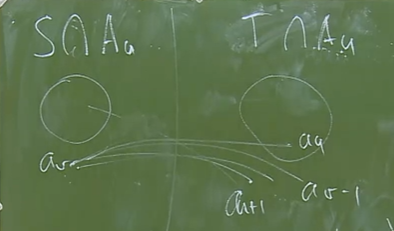
\includegraphics[height=4cm]{images/87-92_ineq.png}}
\end{figure}

% \newpage

\setcounter{section}{87}
\section{Min cost flow: постановка задачи. Алгоритм поиска потока величины k минимальной стоимости (б/д). Асимптотика.}

\begin{figure}[!htb]
   \begin{minipage}{.5\textwidth}
     \centering
     \includegraphics[height = 2 cm]{images/87-92_min-cost}
     \caption{Пример, что такое стоимость}
   \end{minipage}\hfill
    \begin{minipage}{.5\textwidth}
     \centering
     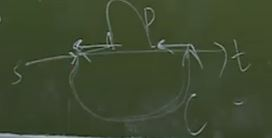
\includegraphics[height = 2 cm]{images/87-92_90_min}
     \caption{Что такое P, C}
   \end{minipage}
\end{figure}

% \includegraphics[height=2cm]{87-92_min-cost}

Таким образом, у нас появляются кроме вместимости потоков стоимости, т.е. сколько нам надо заплатить за пропуск одной единицы потока. Цель: либо фиксированная величина потока, либо максимально возможная при минимальной стоимости (первое: min cost k-flow, второе: min cost max-flow); таким образом, первая задача более общая, чем вторая.

Алгоритм поиска min-cost k-flow: k раз найдём в остаточной сети путь минимальной стоимости, протолкнём единицу потока сквозь него на каждом шаге. Тут dfs не поможет, нужна уже Дейкстра или что-то типа того. Но тут уже возникают рёбра отрицательного веса, из-за чего Дейкстру сходу применить не получится, поэтому по умолчанию применяем Форда-Беллмана + боремся с отрицательными циклами.

Считаем, что в исходной сети нет отрицательных циклов. Но доказывается, что добавление вот этой единички потока никогда не создаст отрицательных циклов (утв. 2).

Асимптотика: $O(k \cdot Ford-Bellman) = O(k VE)$

\setcounter{section}{88}
\section{Критерий минимальности стоимости потока величины k.}

\textbf{Утверждение 2}. Пусть f - поток величины k. Тогда f - min cost k flow тогда и только тогда, когда в остаточной сети $G_f$ нет отрицательных циклов.

$\blacktriangle$
$\Rightarrow$: Очевидно, если в $G_f$ есть отрицательный цикл, то по нему можно пустить часть потока, стоимость уменьшится, величина потока - нет, противоречие.

$\Leftarrow$:  Предположим обратное, f - не min cost k flow, тогда пусть f' - настоящий min cost k flow. Тогда рассмотрим новый поток $g = f' - f$, т.е. на каждом ребре мы рассматриваем разность: $g(e) = f'(e) - f(e)$. Тогда g - поток, притом поток величины ноль; по сути это несколько циклов, где постоянно ходит товар (циркуляция), его стоимость отрицательна, но тогда хотя бы один из циклов отрицательный: противоречие.
$\blacksquare$

\setcounter{section}{89}
\section{Корректность алгоритма поиска min cost k-flow в отсутствие отрицательных циклов.}

\textbf{Утверждение}. Алгоритм поиска min cost k flow после i итераций находит min cost i flow, если в исходном графе G не было отрицательных циклов. 

$\blacktriangle$
$f_0$ - min cost 0 flow. База доказана.
Тогда рассмотрим переход от $f_i$ к $f_{i+1}$: мы просто берём старый поток и остаточную сеть, проталкиваем вдоль неё по потоку поток размера 1, делаем переход. Тогда осталось доказать, что после этого шага мы не создадим отрицательных циклов + воспользуемся критерием минимальности. 

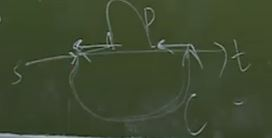
\includegraphics[height = 2 cm]{images/87-92_90_min}

Предположим, что в $G_{f_{i+1}}$ появился отрицательный цикл. Он может появиться только если новый поток использует рёбра, обратные к добавленному потоку. Тогда P + C - путь из s в t в $G_{f_i}$ веса меньше чем P (смотри рисунок 2). $cost (C) < 0 \Rightarrow cost(P + C) < cost (P)$. Таким образом, мы либо нашли путь из s в t меньшей стоимости, либо у нас есть путь + отрицательный цикл, что противоречит либо тому, что P - не кратчайший, либо, что был отрицательный цикл. Противоречие, значит, отрицательных циклов в $G_{f_{i+1}}$ нет.
$\blacksquare$

\setcounter{section}{90}
\section{Потенциалы Джонсона. Поиск min cost k-flow с помощью алгоритма Дейкстры.}

\textbf{Идея}: хотим оптимизировать всё, что было выше, используя Дейкстру.

\textbf{Потенциалы Джонсона (алгоритм Дейкстры-Джонсона)} Пусть $\varphi: V \rightarrow \mathbb{Z}$ - потенциальная функция (некоторая функция из множество вершин в множество целых чисел). Тогда мы можем переопределить стоимости всех рёбер: $cost_\varphi (u, v) = cost(u, v) + \varphi(u) - \varphi(v)$. Это преобразование не меняет кратчайших путей: так как мы рассматривам путь из s в t, то складывая все новые косты, слагаемые взаимоуничтожаются, и значит, новый путь - это старый $+ \varphi(s) - \varphi(t)$, что фиксированно для всех путей из s в t. 

Теперь мы хотим при помощи этой потенциальной функции добиться того, чтобы все веса стали неотрицательными: $cost_\varphi (u, v) \geqslant 0$ $\forall u, v \in G_f$. 

Форд-Беллмана запускаем в самом начале: FB из s, $\varphi(v) = dist(s, v)$ - потенциальная функция. Тогда $cost_\varphi (u, v) \geqslant 0$ $\forall u, v \in G$. Это то же самое, что $cost(u, v) + dist(s, u) - dist(s, v) \geqslant 0$ $\Leftrightarrow$ $dist(s, v) \leqslant cost(u, v) + dist(s, u)$. Но это уже очевидно из того, что dist(s, v) - кратчайший путь (он либо вот такой же - путь от s до u и потом от u до v, либо где-то есть ещё более короткий путь).

Запустим Дейкстру на G с весовой функцией $cost_\varphi$. Кратчайший путь от s до t имеет вес 0 в этом графе + проходит только по нулевым рёбрам. Это верно, т.к. если (u, v) - ребро на кратчайшем пути из s в t в $cost_\varphi$, то оно так же лежало на кратчайшем пути из s в t на $cost$. Но тогда $dist(s, u) + cost(u, v) = dist(s, v)$ $\Rightarrow$ $cost_\varphi(u, v) = 0$.

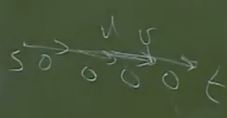
\includegraphics[]{images/87-92_null_path0}

Тогда проталкиваем по этому пути единичку. Появляются/пропадают некоторые рёбра, но если слева направо вес ноль, то справа налево (у обратного ребра) вес тоже ноль. Тогда, получается, отрицательных рёбер не появилось, когда мы протолкнули единичку. Но это верно только для первой итерации, где нули. Но дальше так не проканает: придётся обновлять потенциалы.

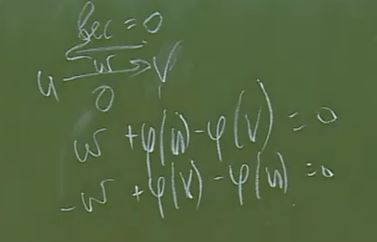
\includegraphics[height=3cm]{images/87-92_null_path}

Пусть $\psi (v) = dist_{cost_\varphi}(s, v)$ - расстояние, которое находит Дейкстра, в сети с $cost_\varphi$. Тогда обновляем потенциалы. Тогда находим с помощью Дейкстры новые потенциалы, и работаем уже с ними. При переходе к новой сети на проталкивании снова будут рёбра нулевого веса, таким образом, отрицательные рёбра никогда не появятся.

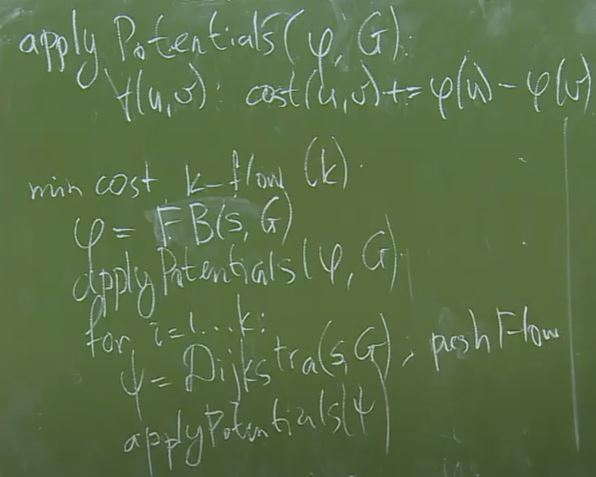
\includegraphics[]{images/87-92_potentials}

Обновление: $\varphi(v) += \psi(v)$

Асимптотика: $VE$ (Форд-Беллман) $+ kV^2$ (или $Elog(V)$, в зависимости от плотности графа) - Дейкстра. Если же в исходном графе не было отрицательных рёбер, то первый Форд-Беллман так же может быть Дейкстрой.

\textbf{Замечание}. Для min cost max flow берём $k = \infty$, если Дейкстра не находит пути, то делает break.

\setcounter{section}{91}
\section{Задача о назначениях. Решение сведением к потоковой задаче.}

\textbf{Условие}. Есть взвешенный полный двудольный граф (на самом деле, может быть и не полным), на каждом ребре по весу. Надо найти совершенное паросочетание минимального веса (в долях по n вершин, размер паросочетания - n). По сути - найти биекцию из левой доли в правую. Название возникло из того, что есть n работников, ресурсы, которые они тратят, n задач, которые они должны выполнить.

Идея аналогична алгоритму Хопкрофта-Карпа: проведём такие же рёбра из s в левую долю, из t в правую, у них capacity 1, косты нулевые. 

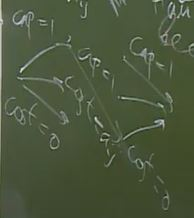
\includegraphics[]{images/87-92_tasks}

Вот мы и свели. Тогда через Дейкстру это будет кубическая асимптотика, так как мы n раз запускаем Дейкстру (в случае полноты графа лучше писать Дейкстру за $n^2$)